\documentclass[11pt,a4paper]{article}

% Packages
\usepackage[utf8]{inputenc}
\usepackage[T1]{fontenc}
\usepackage{CJKutf8}
\usepackage[margin=1in]{geometry}
\usepackage{amsmath,amssymb,amsthm}
\usepackage{graphicx}
\usepackage{subcaption}
\usepackage{hyperref}
\usepackage{listings}
\usepackage{xcolor}
\usepackage{booktabs}
\usepackage{enumitem}
\usepackage{fancyhdr}
\usepackage{pgfplots}


% Code listing style
\lstset{
    basicstyle=\ttfamily\small,
    breaklines=true,
    frame=single,
    numbers=left,
    numberstyle=\tiny\color{gray},
    keywordstyle=\color{blue},
    commentstyle=\color{green!60!black},
    stringstyle=\color{red},
    showstringspaces=false,
    tabsize=4
}

% Header and footer
\pagestyle{fancy}
\fancyhf{}
\lhead{COMP4901B - Large Language Models}
\rhead{Assignment 1}
\cfoot{\thepage}
\setlength{\parindent}{0pt}
\pgfplotsset{compat=1.18}
\setlength{\parskip}{1em}

% Title information
\title{
    \textbf{COMP4901B: Large Language Models} \\
    \vspace{0.5em}
    \Large Assignment 3 Report
}
\author{HE, Wenqian \\ Student ID: 20860896}
\date{\today}

\begin{document}

\maketitle


\section{Part 1 — VLLM Inference Implementation}

\begin{figure}[h]
    \centering
    \includegraphics[width=0.8\textwidth]{figures/part1.png}
    \caption{VLLM Inference}
    \label{fig:vllm_inference}
\end{figure}

\subsection{Implementation}

\textbf{\texttt{format\_prompts()}} I followed the all instructions to implement this function. The quesiton is formatted using specified prompt template by default, then the formatted prompt is applied chat template from tokenizer with optional system message unless exception occurs, otherwise the raw formatted prompt without chat template is used.

\textbf{\texttt{run\_inference()}} I followed the all instructions to implement this function. I pass all necessary parameters to LLM engine and sampling parameters. Specially, If the number of rollouts is greater than 1, but temperature is 0.0, the temperature is increased to 0.6 by default to avoid deterministic output. If the number of rollouts is 1, the temperature is set to 0.0 to avoid stochastic output. Otherwise the temperature is set to the specified temperature.

\subsection{Answer the question}

We need temperature > 0 when generating multiple rollouts because when temperature is 0, the model will generate the same output for each rollout, then there is no meaning to generate multiple rollouts. So we should set temperature > 0 to generate diverse outputs.


\section{Part 2 — Answer Verification Implementation}

\begin{figure}[h]
    \centering
    \includegraphics[width=0.8\textwidth]{figures/part2.png}
    \caption{Answer Verification}
    \label{fig:answer_verification}
\end{figure}

\newpage
\subsection{Implementation}

\begin{lstlisting}[language=Python]
BOX_PATTERN = r'\\boxed\{([^}]+)\}'
NUMBER_PATTERN = r'(-?(?:\d{1,3}(?:,\d{3})*|\d+)(?:\.\d+)?)'
\end{lstlisting}

\textbf{\texttt{extract\_solution()}:} I first try to extract the answer in boxed format using the pattern \texttt{BOX\_PATTERN}, then if not found, I try to extract the answer in number format using the pattern \texttt{NUMBER\_PATTERN}. The last extracted answer is returned without commas and dollar signs. If both failed, I return None. 

\textbf{\texttt{compute\_score()}:} I casted the extracted answer and ground truth to float and back to string to compare the values. This operation is performed in try-except block to handle non-numeric values. If the comparison is successful, it returned the comparison result otherwise 0 is returned.

\subsection{Derivation of the pass@k metric}

\begin{align*}
    \text{pass@k} &= P(\text{at least one correct}) \\
    &= 1 - P(\text{all are wrong}) \\
    &= 1 - \frac{\binom{n-c}{k}}{\binom{n}{k}} \\
    &= 1 - \frac{(n-c)!}{k!(n-c-k)!} \times \frac{k!(n-k)!}{n!} \\
    &= 1 - \frac{(n-c-k+1)(n-c-k+2)\cdots(n-c)}{(n-k+1)(n-k+2)\cdots(n)} \\
    &= 1 - \prod_{i=1}^{k} \frac{n-c-k+i}{n-k+i}
\end{align*}

\subsection{Answer the question}

\begin{lstlisting}
ratios = np.arange(n-c-k+1, n-c+1) / np.arange(n-k+1, n+1)
pass_at_k_values[i] = 1 - np.prod(ratios)
\end{lstlisting}

The numerical stability is achieved by using the product formulation of the pass@k metric. I created a 1d array of \[n-c-k+1, n-c-k+2, \cdots, n-c\] and a 1d array of \[n-k+1, n-k+2, \cdots, n\] then divide the corresponding elements to get the 1d array of ratios. Then the pass@k is 1 minus the product of the ratios. This avoids the computation of large factorials and division of large numbers.

\newpage
\section{Part 3 — LoRA Training Implementation}

\begin{lstlisting}[language=Python]
def _resolve_lora_target_modules(self) -> List[str]:
    VALID_TARGETS_BY_MODEL = {
        "qwen3": {"q_proj", "k_proj", "v_proj", "o_proj", "gate_proj", "up_proj", "down_proj"},
        "llama": {'o_proj', 'k_proj', 'up_proj', 'gate_proj', 'v_proj', 'q_proj', 'down_proj'},
        "mistral": {'k_proj', 'o_proj', 'down_proj', 'q_proj', 'up_proj', 'gate_proj', 'v_proj'},
        "opt": {'k_proj', 'q_proj', 'fc1', 'v_proj', 'out_proj', 'fc2'}
    }
    
    model_type: str = self.model.config.model_type
                    
    if self.lora_args.lora_target_modules:
        targets = set(self.lora_args.lora_target_modules)
    elif model_type in VALID_TARGETS_BY_MODEL:
        targets = VALID_TARGETS_BY_MODEL[model_type]
    else:
        raise ValueError(f"No valid target modules found for model type: {model_type}")
        
    available_modules = {name.split(".")[-1] for name, module in self.model.named_modules() if isinstance(module, nn.Linear)}

    assert targets <= available_modules, f"Invalid target modules: {targets} not in {available_modules}"
    valid_targets = list(targets)
    
    return valid_targets
\end{lstlisting}

\subsection{Detect architecture and select target modules}

I use \texttt{self.model.config.model\_type} to detect the architecture of the model. I downloaded \texttt{Qwen/Qwen3-0.6B}, \texttt{unsloth/Llama-3.2-1B}, \texttt{unsloth/mistral-7b-bnb-4bit} and \newline
\texttt{facebook/opt-125m} models from Hugging Face, then printed the model type string, model architecture, and linear module names. Then I picked the name of linear modules in decoder layers for each model. They are the default valid target modules for forementioned models if no target modules are specified. Details can be found in the \texttt{scripts/model.ipynb} file.

\subsection{Answer the question}
In decoder-only transformer models, the attention layers are used to correlate different parts of the input sequence, i.e. attend to appropriate positions. The FFN layers are used to store the knowledge, such as math operation knowledge. Finetuning lora on attention and FFN layers can help the model focus on the important numbers and quesiton intention keywords for GSM8K-like math problems, then match the learned patterns for each token in FFN layers to perform math reasoning. 

If we only apply lora to attention layers, although it might improve the model's attention on some important number of keywords, but it cannot learn new patterns, such as for which kind of question should it apply division or multiplication. 

Moreover, since the model cannot learn new pattern, it might not be able to extract better features in lower layers through FFN, then higher attention layers cannot pay attention to good positions since they are not similar in terms of features, even though they might relevant in eyes of humans.


\section{Part 4 — Part 4 — Self-Training Execution}
\subsection{Training Configuration Summary}
I trained the models for 4 iterations using the following configuration, which is also the default configuration.
\begin{lstlisting}
NUM_ITERATIONS=4
MAX_TOKENS=512
N_ROLLOUTS=8
ENABLE_THINKING=false
N_QUERIES=2000

LEARNING_RATE=2e-5
TOTAL_BATCH_SIZE=128
NUM_EPOCHS=1
SAVE_STEPS=30
LORA_R=64
\end{lstlisting}

\subsection{Metrics}

See table \ref{tab:metrics} for the metrics across training iterations and figure \ref{fig:accuracy_plot} for the accuracy improvement across iterations. The number of coorect solutions found and accuracy is collected by \texttt{run\_gsm8k\_eval.sh} script with single rollout. The pass@k metrics are collected by \newline \texttt{run\_gsm8k\_eval.sh} script with multiple rollouts. The training loss is collected in the end of each iteration. Detailed log can be found at \texttt{ckpt/} and \texttt{results/} directories.

\begin{table}[h]
    \centering
    \begin{tabular}{lrrrrrr}
        \toprule
        \textbf{Iteration} & \textbf{\#Correct} & \textbf{Accuracy} & \textbf{Pass@1} & \textbf{Pass@4} & \textbf{Pass@8} & \textbf{Training Loss} \\
        \midrule
        0 (baseline) & 803 & 60.88\% & 0.6070 & 0.7810 & 0.8500 & --- \\
        1 & 838 & 63.53\% & 0.6300 & 0.8020 & 0.8480 & 0.2865 \\
        2 & 841 & 63.76\% & 0.6080 & 0.8130 & \textbf{0.8620} & 0.2874 \\
        3 & 836 & 63.38\% & \textbf{0.6320} & \textbf{0.8030} & 0.8580 & 0.2875 \\
        4 & \textbf{854} & \textbf{64.75\%} & 0.6310 & 0.8040 & 0.8570 & \textbf{0.2862} \\
        \bottomrule
    \end{tabular}
    \caption{Performance metrics across training iterations. Bold values indicate the best performance in each column.}
    \label{tab:metrics}
\end{table}

\subsection{Analysis}

Self-training improves the accuracy from 60.88\% to 64.75\% across 4 iterations. By training on the correct solutions, the model learns what's the potential correct reasoning process that leads to correct answers from the output sampled from the model itself, and tend to generate reasoning process similar to them in the future, therefore solving similar problems more accurately.

\begin{figure}[h]
    \centering
    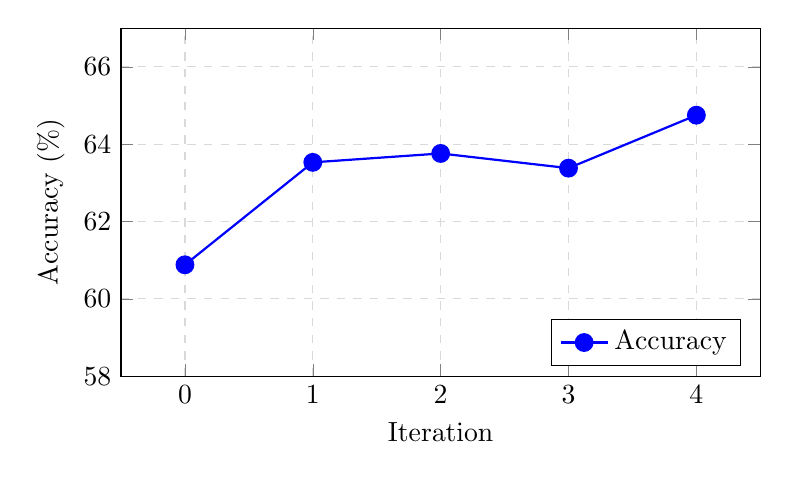
\begin{tikzpicture}
        \begin{axis}[
            width=0.8\textwidth,
            height=6cm,
            xlabel={Iteration},
            ylabel={Accuracy (\%)},
            xmin=-0.5, xmax=4.5,
            ymin=58, ymax=67,
            xtick={0,1,2,3,4},
            ytick={58,60,62,64,66},
            grid=major,
            grid style={dashed,gray!30},
            mark size=3pt,
            legend pos=south east,
        ]
        
        % Accuracy data
        \addplot[
            color=blue,
            mark=*,
            thick,
        ] coordinates {
            (0, 60.88)
            (1, 63.53)
            (2, 63.76)
            (3, 63.38)
            (4, 64.75)
        };
        \addlegendentry{Accuracy}
        
        \end{axis}
    \end{tikzpicture}
    \caption{Accuracy improvement across iterations}
    \label{fig:accuracy_plot}
\end{figure}



\section{Part 5 — Final Evaluation and Analysis}
\subsection{Baseline Evaluation}

The baseline accuracy is 60.88\% as shown in the figure \ref{fig:eval_baseline_1}. The detailed evaluation results can be found at \texttt{results/baseline/} directory.


\subsection{Trained Model Evaluation}

Please see table \ref{tab:hyperparameters} for the evaluation results across different hyperparameter variations and training iterations. The detailed evaluation results can be found at \texttt{results/} directory. All screenshots can be found in the appendix.

\textbf{Ablation Study:} Based on the evaluation results, within one iteration, the best performance is achieved when lowering the batch size to 64, attaining 63.84\% accuracy. The other settings, including decreasing learning rate, increasing learning rate, decreasing queries, increasing queries, increasing batch size, are all worse than the default settings. 

\textbf{Best Performance:} The best performance is achieved by running more iterations on the default settings, which is 64.75\% accuracy.

\begin{table}[h]
    \centering
    \begin{tabular}{lccccr}
        \toprule
        \textbf{Model} & \textbf{Iteration} & \textbf{BSZ} & \textbf{LR} & \textbf{N\_QUERIES} & \textbf{Accuracy} \\
        \midrule
        default & 1 & 128 & 2e-5 & 2000 & 63.53\% \\
        $\downarrow$ lr & 1 & 128 & 1e-5 & 2000 & 61.56\% \\
        $\uparrow$ lr & 1 & 128 & 4e-5 & 2000 & 62.55\% \\
        $\downarrow$ queries & 1 & 128 & 2e-5 & 1500 & 63.31\% \\
        $\uparrow$ queries & 1 & 128 & 2e-5 & 3000 & 62.17\% \\
        $\downarrow$ batch size & 1 & 64 & 2e-5 & 2000 & \textbf{63.84\%} \\
        $\uparrow$ batch size & 1 & 256 & 2e-5 & 2000 & 62.70\% \\
        \midrule
        default iter 1 & 1 & 128 & 2e-5 & 2000 & 63.53\% \\
        default iter 2 & 2 & 128 & 2e-5 & 2000 & 63.76\% \\
        default iter 3 & 3 & 128 & 2e-5 & 2000 & 63.38\% \\
        default iter 4 & 4 & 128 & 2e-5 & 2000 & \textbf{64.75\%} \\
        \bottomrule
    \end{tabular}
    \caption{Hyperparameter ablation study and iterative training results. Bold values indicate best performance within each section.}
    \label{tab:hyperparameters}
\end{table}


\subsection{Analysis}

Please see table \ref{tab:detailed_analysis} for the detailed analysis of the avg@k and pass@k metrics across hyperparameter variations and training iterations. The detailed evaluation results can be found at \texttt{results/} directory. All screenshots can be found in the appendix.

\textbf{Trend:} For avg@k metrics, we can see that for the first iteration, the avg@k tend to be lower as k increase, but in higher iteration, the avg@k tends to be stable or slightly increase. However, for pass@k metrics, we can see that for all iterations, the pass@k tends to be higher as k increase, but higher iteration does not indicate better pass@k metrics. 

\textbf{Gap between avg@k and pass@k metrics:} In baseline model, and also all the trained models, there is a gap between avg@k and pass@k metrics, indicating although the accuracy may not be high enough, we by trying multiple times, the model is still able to provide correct answer with high probability, even for some cases, the correct answer is not the first one. Therefore, pass@k metrics with high k is the potential value of the accuracy to achieve by the model after self-training.

\textbf{Comparison before and after training:} All metrics after training are better than the baseline (for default settings), indicating that self-training is effective. By training on the correct solutions, the model learns what's the potential correct reasoning process that leads to correct answers from the output sampled from the model itself, and tend to generate reasoning process similar to them in the future, therefore solving similar problems more accurately.

\textbf{Diversity and Reliability:} When training with default settings within one iteration, the improvement of pass@k metrics is lower and lower as k increase, although avg@k metrics improves with roughly fixed amount. This indicates that the model is more reliable in general to provide correct answer without extensive retry, but the output is less diverse, less likely to get correct answer surprisingly after multiple attempts. Since pass@k metrics improved less significantly compared to avg@k metrics, the model is less diverse after training. 

\begin{table}[h]
    \centering
    \begin{tabular}{lcrrrrrr}
        \toprule
        \textbf{Model} & \textbf{Iter} & \textbf{avg@1} & \textbf{avg@4} & \textbf{avg@8} & \textbf{pass@1} & \textbf{pass@4} & \textbf{pass@8} \\
        \midrule
        baseline & 0 & 0.6070 & 0.5962 & 0.5966 & 0.6070 & 0.7810 & 0.8500 \\
        \midrule
        default & 1 & \textbf{0.6300} & 0.6148 & \textbf{0.6146} & \textbf{0.6300} & 0.8020 & 0.8480 \\
        $\downarrow$ lr & 1 & 0.6230 & 0.6110 & 0.6095 & 0.6230 & 0.7940 & 0.8480 \\
        $\uparrow$ lr & 1 & 0.6030 & 0.6067 & 0.6089 & 0.6030 & 0.7830 & 0.8330 \\
        $\downarrow$ queries & 1 & 0.6090 & 0.6072 & 0.6125 & 0.6090 & 0.7880 & 0.8440 \\
        $\uparrow$ queries & 1 & 0.6110 & 0.6140 & 0.6121 & 0.6110 & \textbf{0.8030} & 0.8480 \\
        $\downarrow$ batch size & 1 & 0.6260 & \textbf{0.6152} & 0.6134 & 0.6260 & 0.8020 & \textbf{0.8500} \\
        $\uparrow$ batch size & 1 & 0.6170 & 0.6098 & 0.6076 & 0.6170 & 0.7880 & 0.8390 \\
        \midrule
        default iter 1 & 1 & 0.6300 & 0.6148 & 0.6146 & 0.6300 & 0.8020 & 0.8480 \\
        default iter 2 & 2 & 0.6080 & 0.6302 & 0.6300 & 0.6080 & \textbf{0.8130} & \textbf{0.8620} \\
        default iter 3 & 3 & \textbf{0.6320} & \textbf{0.6360} & 0.6309 & \textbf{0.6320} & 0.8030 & 0.8580 \\
        default iter 4 & 4 & 0.6310 & 0.6330 & \textbf{0.6350} & 0.6310 & 0.8040 & 0.8570 \\
        \bottomrule
    \end{tabular}
    \caption{Detailed analysis of average and pass@k metrics across hyperparameter variations and training iterations. Bold values indicate best performance within each section.}
    \label{tab:detailed_analysis}
\end{table}

\clearpage
\section{Appendix}

\subsection{Ablation Study Evaluation Results}

\begin{figure}[h!]
    \centering
    \begin{subfigure}[b]{0.48\textwidth}
        \centering
        \includegraphics[width=\textwidth]{figures/eval_baseline_1.png}
        \caption{1 rollout}
        \label{fig:eval_baseline_1}
    \end{subfigure}
    \hfill
    \begin{subfigure}[b]{0.48\textwidth}
        \centering
        \includegraphics[width=\textwidth]{figures/eval_baseline_8.png}
        \caption{8 rollouts}
        \label{fig:eval_baseline_8}
    \end{subfigure}
    \caption{Baseline evaluation results with different numbers of rollouts}
    \label{fig:eval_baseline}
\end{figure}



\begin{figure}[h!]
    \centering
    \begin{subfigure}[b]{0.48\textwidth}
        \centering
        \includegraphics[width=\textwidth]{figures/eval_lr_1e-5_1.png}
        \caption{1 rollout}
        \label{fig:eval_lr_1e-5_1}
    \end{subfigure}
    \hfill
    \begin{subfigure}[b]{0.48\textwidth}
        \centering
        \includegraphics[width=\textwidth]{figures/eval_lr_1e-5_8.png}
        \caption{8 rollouts}
        \label{fig:eval_lr_1e-5_8}
    \end{subfigure}
    \caption{Decreasing learning rate to 1e-5 evaluation results with different numbers of rollouts}
    \label{fig:eval_lr_1e-5}
\end{figure}

\begin{figure}[h!]
    \centering
    \begin{subfigure}[b]{0.48\textwidth}
        \centering
        \includegraphics[width=\textwidth]{figures/eval_lr_4e-5_1.png}
        \caption{1 rollout}
        \label{fig:eval_lr_4e-5_1}
    \end{subfigure}
    \hfill
    \begin{subfigure}[b]{0.48\textwidth}
        \centering
        \includegraphics[width=\textwidth]{figures/eval_lr_4e-5_8.png}
        \caption{8 rollouts}
        \label{fig:eval_lr_4e-5_8}
    \end{subfigure}
    \caption{Increasing learning rate to 4e-5 evaluation results with different numbers of rollouts}
    \label{fig:eval_lr_4e-5}
\end{figure}

\begin{figure}[h!]
    \centering
    \begin{subfigure}[b]{0.48\textwidth}
        \centering
        \includegraphics[width=\textwidth]{figures/eval_q_1500_1.png}
        \caption{1 rollout}
        \label{fig:eval_queries_1500_1}
    \end{subfigure}
    \hfill
    \begin{subfigure}[b]{0.48\textwidth}
        \centering
        \includegraphics[width=\textwidth]{figures/eval_q_1500_8.png}
        \caption{8 rollouts}
        \label{fig:eval_q_1500_8}
    \end{subfigure}
    \caption{Decreasing queries to 1500 evaluation results with different numbers of rollouts}
    \label{fig:eval_q_1500}
\end{figure}

\begin{figure}[h!]
    \centering
    \begin{subfigure}[b]{0.48\textwidth}
        \centering
        \includegraphics[width=\textwidth]{figures/eval_q_3000_1.png}
        \caption{1 rollout}
        \label{fig:eval_q_3000_1}
    \end{subfigure}
    \hfill
    \begin{subfigure}[b]{0.48\textwidth}
        \centering
        \includegraphics[width=\textwidth]{figures/eval_q_3000_8.png}
        \caption{8 rollouts}
        \label{fig:eval_q_3000_8}
    \end{subfigure}
    \caption{Increasing queries to 3000 evaluation results with different numbers of rollouts}
    \label{fig:eval_q_3000}
\end{figure}

\begin{figure}[htbp]
    \centering
    \begin{subfigure}[b]{0.48\textwidth}
        \centering
        \includegraphics[width=\textwidth]{figures/eval_bsz_64_1.png}
        \caption{1 rollout}
        \label{fig:eval_bsz_64_1}
    \end{subfigure}
    \hfill
    \begin{subfigure}[b]{0.48\textwidth}
        \centering
        \includegraphics[width=\textwidth]{figures/eval_bsz_64_8.png}
        \caption{8 rollouts}
        \label{fig:eval_bsz_64_8}
    \end{subfigure}
    \caption{Decreasing batch size to 64 evaluation results with different numbers of rollouts}
    \label{fig:eval_bsz_64}
\end{figure}

\begin{figure}[tbp]
    \centering
    \begin{subfigure}[b]{0.48\textwidth}
        \centering
        \includegraphics[width=\textwidth]{figures/eval_bsz_256_1.png}
        \caption{1 rollout}
        \label{fig:eval_bsz_256_1}
    \end{subfigure}
    \hfill
    \begin{subfigure}[b]{0.48\textwidth}
        \centering
        \includegraphics[width=\textwidth]{figures/eval_bsz_256_8.png}
        \caption{8 rollouts}
        \label{fig:eval_bsz_256_8}
    \end{subfigure}
    \caption{Increasing batch size to 256 evaluation results with different numbers of rollouts}
    \label{fig:eval_bsz_256}
\end{figure}

\clearpage

\subsection{Multi-Iteration Evaluation Results}

\begin{figure}[h!]
    \centering
    \begin{subfigure}[b]{0.48\textwidth}
        \centering
        \includegraphics[width=\textwidth]{figures/eval_default_multi_iter_1_1.png}
        \caption{1 rollout}
        \label{fig:eval_default_multi_iter_1_1}
    \end{subfigure}
    \hfill
    \begin{subfigure}[b]{0.48\textwidth}
        \centering
        \includegraphics[width=\textwidth]{figures/eval_default_multi_iter_1_8.png}
        \caption{8 rollouts}
        \label{fig:eval_default_multi_iter_1_8}
    \end{subfigure}
    \caption{Default 1 iteration evaluation results with different numbers of rollouts}
    \label{fig:eval_default_multi_iter_1}
\end{figure}

\begin{figure}[h!]
    \centering
    \begin{subfigure}[b]{0.48\textwidth}
        \centering
        \includegraphics[width=\textwidth]{figures/eval_default_multi_iter_2_1.png}
        \caption{1 rollout}
        \label{fig:eval_default_multi_iter_2_1}
    \end{subfigure}
    \hfill
    \begin{subfigure}[b]{0.48\textwidth}
        \centering
        \includegraphics[width=\textwidth]{figures/eval_default_multi_iter_2_8.png}
        \caption{8 rollouts}
        \label{fig:eval_default_multi_iter_2_8}
    \end{subfigure}
    \caption{Default 2 iterations evaluation results with different numbers of rollouts}
    \label{fig:eval_default_multi_iter_2}
\end{figure}

\begin{figure}[h!]
    \centering
    \begin{subfigure}[b]{0.48\textwidth}
        \centering
        \includegraphics[width=\textwidth]{figures/eval_default_multi_iter_3_1.png}
        \caption{1 rollout}
        \label{fig:eval_default_multi_iter_3_1}
    \end{subfigure}
    \hfill
    \begin{subfigure}[b]{0.48\textwidth}
        \centering
        \includegraphics[width=\textwidth]{figures/eval_default_multi_iter_3_8.png}
        \caption{8 rollouts}
        \label{fig:eval_default_multi_iter_3_8}
    \end{subfigure}
    \caption{Default 3 iterations evaluation results with different numbers of rollouts}
    \label{fig:eval_default_multi_iter_3}
\end{figure}

\begin{figure}[h!]
    \centering
    \begin{subfigure}[b]{0.48\textwidth}
        \centering
        \includegraphics[width=\textwidth]{figures/eval_default_multi_iter_4_1.png}
        \caption{1 rollout}
        \label{fig:eval_default_multi_iter_4_1}
    \end{subfigure}
    \hfill
    \begin{subfigure}[b]{0.48\textwidth}
        \centering
        \includegraphics[width=\textwidth]{figures/eval_default_multi_iter_4_8.png}
        \caption{8 rollouts}
        \label{fig:eval_default_multi_iter_4_8}
    \end{subfigure}
    \caption{Default 4 iterations evaluation results with different numbers of rollouts}
    \label{fig:eval_default_multi_iter_4}
\end{figure}



\end{document}